\documentclass{article}

\usepackage[english]{babel}
\usepackage[a4paper,top=2cm,bottom=2cm,left=3cm,right=3cm,marginparwidth=1.75cm]{geometry}
\usepackage[backend=biber, sorting=nyt, style=authoryear-ibid]{biblatex}
%\bibliographystyle{agsm}
%\let\cite\textcite

\usepackage{amsmath}
\usepackage{csquotes}
\usepackage{graphicx}
\graphicspath{ {figures/} }
\usepackage[colorlinks=true, allcolors=blue]{hyperref}
\usepackage{parskip}
\usepackage{array}
\usepackage{multirow}
\usepackage{fontspec}
\usepackage{fontawesome5}
%\newcommand{\faWindows}{\FA\symbol{"F17A}}
%\newcommand{\faLinux}{\FA\symbol{"F17C}}
%\newcommand{\faApple}{\FA\symbol{"F179}}

%\bibliography{references}
\addbibresource{references.bib}

\title{Mockingjay Assignment Literature Review}
\author{Stuart Kingham}

\begin{document}
\maketitle

\begin{abstract}
Literature review.
\end{abstract}

\newpage
\tableofcontents
\listoffigures
\listoftables
\pagenumbering{roman}
\pagenumbering{arabic}
\newpage

\section{Introduction}

\textbf{Citations}

Cite using:
\begin{enumerate}
\item \textbf{citetitle\{Smith:2012jd\}}: \citetitle{Berdajs:2010}
\item \textbf{parencite\{Smith:2012qr\}}: A citation command in parentheses: \parencite{Berdajs:2010}.
\item \textbf{textcite\{Smith:2024jd\}}: For use in the flow of text: As \textcite{Berdajs:2010} said \dots
\item \textbf{autocite\{Peixoto:2023\}}: A citation command which automatically switches style depending on
  location and the option setting in the package declaration (see line 12 in the LaTeX source code). In this
  case, it produces a citation in parentheses: \autocite{Peixoto:2023}.
\end{enumerate}


\subsection{Nobody loves me}

In light of the concerns raised in the Harvard Business Review article, this report aims to address the critical issues surrounding cybersecurity oversight by boards. The challenges outlined, including the disconnect between boards and CISOs, the focus on protection over resilience, the perception of cybersecurity as a technical topic, the need for cybersecurity expertise in board composition, and the imperative of making cybersecurity a continuous priority, underscore the urgency for a more strategic and proactive approach. This report will delve into the specific aspect of malware attacks and process injection techniques on Windows, offering insights and recommendations to enhance board-level discussions and decisions in the ever-evolving landscape of cybersecurity threats.

\subsubsection{\textcite{Milica:2023}}
\textbf{\citetitle{Milica:2023}}: Headlines increasingly highlight the consequences of poor cybersecurity practices. Board members with cybersecurity experience are trying to get their fellow members’ attention on it. And board members want to provide oversight, even though they just don’t have the right questions to ask. Boards need to discuss their organization’s cybersecurity-induced risks and evaluate plans to manage those risks. With the right conversations about keeping the company resilient, they can take the next step to provide adequate cybersecurity oversight.

The Harvard Business Review article discusses the challenges faced by boards in providing effective oversight for cybersecurity. Despite acknowledging cybersecurity as a priority, boards often fall short in fostering organizational resilience against cyberattacks. A survey of 600 board members reveals a significant gap between board perceptions and the reality of cyber risk preparedness.

In light of the concerns raised in the Harvard Business Review article, this report aims to address the critical issues surrounding cybersecurity oversight by boards. The challenges outlined include:

\begin{itemize}
  \item \textbf{Disconnect Between Boards and CISOs:}
        \begin{enumerate}
          \item Only 69\% of board members align with their Chief Information Security Officers (CISOs).
          \item Limited interaction between boards and CISOs impedes meaningful cybersecurity discussions.
          \item Communication gaps and misalignment hinder progress in cybersecurity.
        \end{enumerate}
        
  \item \textbf{Focus on Protection Over Resilience:}
        \begin{enumerate}
          \item Boards tend to prioritize cyber protection despite a high perceived risk.
          \item Investments in protection may not be directed to the most critical areas.
          \item The article advocates a shift in focus towards organizational resilience to minimize damage and recovery time.
        \end{enumerate}
        
  \item \textbf{Cybersecurity as a Technical Topic:}
        \begin{enumerate}
          \item Boards view cybersecurity primarily as a technical issue rather than an organizational imperative.
          \item Limited time in board meetings makes it challenging to address the nuances of cybersecurity.
          \item Shifting the discussion from technical to management challenges is crucial for effective oversight.
        \end{enumerate}
        
  \item \textbf{Board Composition and Expertise:}
        \begin{enumerate}
          \item Many boards lack cybersecurity expertise, relying on seasoned executives with other backgrounds.
          \item The SEC proposes explicit cybersecurity recommendations for boards, necessitating expertise inclusion.
          \item Board composition may need to change to incorporate members with cybersecurity knowledge.
        \end{enumerate}
        
  \item \textbf{Priority and Commitment:}
        \begin{enumerate}
          \item A quarter of boardrooms do not view cybersecurity as a priority, with infrequent discussions.
          \item Making cybersecurity a true priority requires ongoing commitment, regular updates, and personal interest from board members.
          \item Directors' personal actions send messages to senior leaders about the importance of cybersecurity.
        \end{enumerate}
\end{itemize}

This report will delve into the specific aspect of malware attacks and process injection techniques on Windows, offering insights and recommendations to enhance board-level discussions and decisions in the ever-evolving landscape of cybersecurity threats.

\subsection{CISO Challenges in Cybersecurity Oversight by Boards}

\subsubsection{Are we spending enough}

\subsubsection{\textcite{FBI:2023}}
\textbf{\citetitle{FBI:2023}}: 


\subsubsection{\textcite{Hiscox:2022}}
\textbf{\citetitle{Hiscox:2022}}: 



% Section 2 is a literature review of HBCI methods and endpoint security that is typically relied upon to prevent these types of attack.  We will then look at methods a identifying these attacks and look at the likelihood of Endpoint Security products of identifying the attack

% introduce EDRs and how they are used to protect organisations

% introduce process injection attacks: MITRE, and NT process attacks

% how do EDRs

\section{Process Injection Techniques as Malware Attacks on Windows}
% \section{Host-based code injection attack (HBCIA) techniques}

\subsubsection{\textcite{Ghizzoni:2004} Initial technique developed by Microsoft for legal uses}
\textbf{\citetitle{Ghizzoni:2004}}: MS Patent. Many software programs and computer-oriented tools and techniques monitor and analyze executable programs and modules. In many instances, these software programs, tools, and techniques may need to control another program (i.e., “target process”), change a target process' behavior with the target process being unaware of the change in control or behavior, or determine how the target process will interact with other programs and the operating system in which the target process will be run.

For example, anti-virus software needs to map into the target process and determine what the target process will do when it is activated. Debuggers are used to detect, locate, and correct logical or syntactical errors in the target process. They allow a programmer to step through a target process, examine the data, and monitor conditions (such as variables) in the target process. Profilers analyze a target process and determine the time that the process spends in various parts the process during execution. This is often used to determine which API (Application Programming Interface) calls are taking up time. Security check tools verify that a user is authorized to execute a particular process or that a target process is allowed to run a particular task. API interception techniques intercept program calls sent to a target process or sent from a target process. This requires mapping into the target process at the beginning of the process' execution and is done for a variety of reasons including testing the target process, profiling, monitoring selected events, and re-directing the API call to another process. Pseudo-localization attempts to anticipate what a target process will do when that process and the process' resources are changed into a different language for operation in different regions of the world.

Many software programs and computer-oriented tools and techniques monitor and analyze executable programs and modules. In many instances, these software programs, tools, and techniques may need to control another program (i.e., “target process”), change a target process' behavior with the target process being unaware of the change in control or behavior, or determine how the target process will interact with other programs and the operating system in which the target process will be run.

For example, anti-virus software needs to map into the target process and determine what the target process will do when it is activated. Debuggers are used to detect, locate, and correct logical or syntactical errors in the target process. They allow a programmer to step through a target process, examine the data, and monitor conditions (such as variables) in the target process. Profilers analyze a target process and determine the time that the process spends in various parts the process during execution. This is often used to determine which API (Application Programming Interface) calls are taking up time. Security check tools verify that a user is authorized to execute a particular process or that a target process is allowed to run a particular task. API interception techniques intercept program calls sent to a target process or sent from a target process. This requires mapping into the target process at the beginning of the process' execution and is done for a variety of reasons including testing the target process, profiling, monitoring selected events, and re-directing the API call to another process. Pseudo-localization attempts to anticipate what a target process will do when that process and the process' resources are changed into a different language for operation in different regions of the world.

\subsubsection{\textcite{Berdajs:2010} API Hooking also used to detect malare}
\textbf{\citetitle{Berdajs:2010}}: When programmers need to modify third-party applications, they frequently do not have access to their source code. In such cases, DLL injection and API hooking are techniques that can be used to modify applications without intervening into their source code. The commonly used varieties of injection and hooking approaches have many practical limitations: they are inconvenient for a programmer to implement, do not work reliably in conjunction with all applications and with certain low-level machine instructions. In this paper we present two novel approaches to DLL injection and API hooking, which we call Debugger-aided DLL injection and Single Instruction Hooking. Our approaches overcome the limitations of the state-of-the art approaches. Despite incurring greater execution times, our approach allows extending of the applications in situations where the comparable approaches fail. As such, it has a notable practical value for beneficial practical applications of injection and hooking approaches, which are present in malware detection programs and computer security tools.



\subsection{Background Reasons for Process Injection}

Process injection refers to different methods employed to deliver malicious code into the memory space of a
running process.  The technique enables attackers to hide the injected code \textit{how?} and evade detection.

In a Windows \faWindows \space environment, attackers rely on a combination of Windows APIs to effect the injection
process \textit{what are these? Are they all the same, can they be categorised?}.

Security solutions are aware of these techniques and have measures to detect and block the injection process based
on the patterns of executed calls in the OS during the infection.  A promenant adveserial challenge by \textbf{EDR}
systems is to set hooks on the NT system API calls within the memory space of every launched process on protected
systems.  These hooks intercept and capture the calling parameters to Windows APIs to identify potentially malicious actions.

The security team at Security Joes looked to ``discover alternative methods to dynamically execute code within
the memory space of Windows processes, without relying on monitored Windows APIs.''  Their process involved
finding trusted Windows libraries that have sections \textit{what is a section and why is it important to this?}
with default protections set as Read-Write-eXecute (RWX).  Code was demonstrated that injected code into various
processes, eliminating the need to execute several Windows API calls usually monitored by security solutions.
As the attack does not directly invoke Windows API calls usually associated with process injection techniques.

Their starting point is a HBCIA \textit{check assumption that the attack is a hollowing out, hence destructive to the host proces - must be better term than host process. If it is destructive, then cannot by HBCI/RBCI; must be an attack} identifying a process with a section that can be attacked.  They then show how they can construct a RBCIA.

\subsubsection{\textcite{Barabosch:2014} Taxonomy of process injection}
\textbf{\citetitle{Barabosch:2014}}: \textit{Formalises HBCIA/RBCIA and key components, attack algorithm taxonomy, prevalence estimation.}  Common goals of malware authors are detection avoidance and gathering of critical information. There exist numerous techniques that help these actors to reach their goals. One especially popular technique is the Host-Based Code Injection Attack (HBCIA). According to our research 63.94\% out of a malware set of 162850 samples use HBCIAs. The act of locally copying malicious code into a foreign process space and subsequently executing it is called a Host-Based Code Injection Attack. In this paper, we define HBCIAs and introduce a taxonomy for HBCIA algorithms. We show that a HBCIA algorithm can be broken down into three steps. In total there are four classes of HBCIA algorithms. Then we examine a huge set of malware samples and estimate the prevalence of HBCIA-employing malware and their target process distribution. Moreover, we analyse Intrusion Prevention System data and show that HBCIA-employing malware prefers network-related processes for its network communication. To the best of our knowledge, we are the first to thoroughly describe and formalize this phenomenon and give an estimation of its prevalence. Thus, we build a solid foundation for future work on this topic.

\textbf{Keywords}: Code injection,  Process injection, Host-based injection, Malware techniques, Targeted injection, Shotgun injection, Concurrent execution, Thread manipulation

Differentiate between HBCI and HBCIA, HBCI \& RBCI.

This paper provides an in-depth analysis of host-based code injection attacks (HBCIAs), which are a popular technique used by malware. Here is a summary of the key points:


HBCIAs involve injecting malicious code into a running process to avoid detection and intercept information. Advantages for malware authors include avoiding detection, privilege escalation, and manipulating security products. Disadvantages include increased complexity and risk of system instability.

An HBCIA consists of three main steps:

\begin{enumerate}
\item selecting a victim process,
\item copying code into the victim process, and
\item executing the injected code.
\end{enumerate}

These steps can be categorized into different classes:

\begin{itemize}
\item Victim Selection:
  \begin{enumerate}
    \item Targeted Injection:
      \begin{itemize}
      \item Malware selects a specific subset of processes to inject into based on an internal target list
      \item Typically injects into critical system processes like explorer.exe
      \item Less suspicious as avoids risky/unnecessary processes
      \end{itemize}
    \item Shotgun Injection:
      \begin{itemize}
        \item Malware blindly injects itself into as many accessible processes as possible
        \item Greedy approach that injects into every process it can access
        \item More suspicious as may accidentally target antivirus or risky processes
     \end{itemize}
 \end{enumerate}

  In summary, targeted injection allows malware to be more careful and selective in choosing processes to inject into, while shotgun injection aggressively injects into anything accessible without consideration for stealth or stability.

  \item Code Execution: Concurrent Execution or Thread Manipulation

    \begin{enumerate}
      \item Concurrent Execution:
        \begin{itemize}
          \item The injected code runs in parallel with the original code in the victim process
          \item Original threads of the victim process continue executing
          \item Additional threads are spawned for the injected code
          \item Victim process exhibits a blend of its original and the injected code's behavior
        \end{itemize}

    \item Thread Manipulation:
        \begin{itemize}
        \item The injected code replaces or blocks the original victim process's thread(s)
        \item Original threads of the victim process do not continue
        \item Victim process exhibits mainly the injected code's behavior
        \item Can render victim process useless
      \end{itemize}
    \end{enumerate}

    In summary, with concurrent execution the victim process still runs its original code along with the injected code, while in thread manipulation the injected code takes over and blocks the original process code from executing.

\end{itemize}


This results in 4 possible HBCIA algorithm classes:

\begin{itemize}
\item TICE: Targeted Injection + Concurrent Execution 
\item TITM: Targeted Injection + Thread Manipulation
\item SICE: Shotgun Injection + Concurrent Execution
\item SITM:  Shotgun Injection + Thread Manipulation (no known malware examples)
\end{itemize}

\textbf{Key findings from malware analysis:}

\begin{itemize}
\item 63.94\% of over 160,000 samples used HBCIAs 
\item Targeted injection and concurrent execution are most popular
\item Preferred victim processes are system processes like explorer.exe and svchost.exe
\item Network communication occurs through different processes than victim processes
\end{itemize}


\iffalse
\fi

\begin{figure}[h]
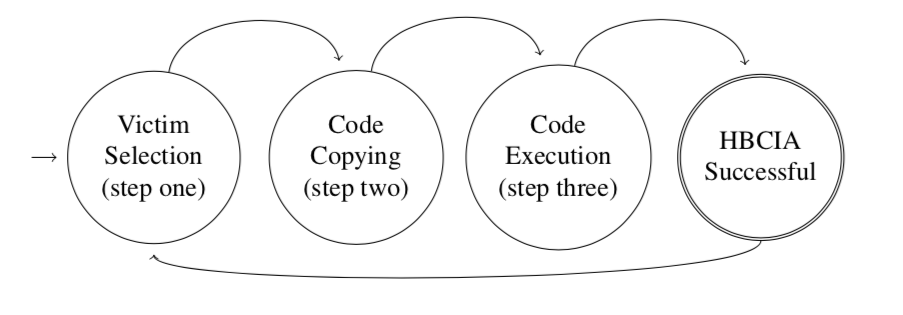
\includegraphics[scale=0.4]{hbcia_3step_algo.png}
\caption{HBCIA Attack Steps \autocite{Barabosch:2014}}
\end{figure}



\subsection{Code Injection Methods}

\subsubsection{\textcite{Oosthoek:2019}}
\textbf{\citetitle{Oosthoek:2019}}: 


\subsubsection{\textcite{Mitre:2017} Twelve Mitre injection techniques}
\textbf{\citetitle{Mitre:2017}}: Adversaries may inject code into processes in order to evade process-based defences as well as possibly elevate privileges. Process injection is a method of executing arbitrary code in the address space of a separate live process. Running code in the context of another process may allow access to the process's memory, system/network resources, and possibly elevated privileges. Execution via process injection may also evade detection from security products since the execution is masked under a legitimate process. 

There are many different ways to inject code into a process, many of which abuse legitimate functionalities. These implementations exist for every major OS but are typically platform specific. 
More sophisticated samples may perform multiple process injections to segment modules and further evade detection, utilizing named pipes or other inter-process communication (IPC) mechanisms as a communication channel. 

\begin{itemize}
\item T1055.001	Dynamic-link Library Injection
\item T1055.002	Portable Executable Injection
\item T1055.003	Thread Execution Hijacking
\item T1055.004	Asynchronous Procedure Call
\item T1055.005	Thread Local Storage
\item T1055.008	Ptrace System Calls
\item T1055.009	Proc Memory
\item T1055.011	Extra Window Memory Injection
\item T1055.012	Process Hollowing
\item T1055.013	Process Doppelgänging
\item T1055.014	VDSO Hijacking
\item T1055.015	ListPlanting
\end{itemize}


\begin{table}[!ht]
  \centering
  \caption{Attack Mitigants \autocite{Mitre:2017}}
\begin{tabular}{ |p{1.2cm}||p{2cm}|p{11.5cm}|  }
  \hline
  \multicolumn{3}{|c|}{PI Mitigation List} \\
  \hline
  ID	& Mitigation & Description \\
  \hline
  M1040	& Behavior Prevention on Endpoint &	Some endpoint security solutions can be configured to block some types of
                                            process injection based on common sequences of behavior that occur during the
                                            injection process. For example, on Windows 10, Attack Surface Reduction (ASR)
                                            rules may prevent Office applications from code injection. [78] \\
  \hline
  M1026 & Privileged Account Management	& Utilize Yama (ex: /proc/sys/kernel/yama/ptrace\_scope) to mitigate ptrace based
                                          process injection by restricting the use of ptrace to privileged users only. Other
                                          mitigation controls involve the deployment of security kernel modules that provide
                                          advanced access control and process restrictions such as SELinux, grsecurity,
                                          and AppArmor. \\
  \hline
\end{tabular}
\label{table: Mitigations}
\end{table}

\begin{table}[!ht]
\centering
\caption{Injection Detection Methods \autocite{Mitre:2017}}
\begin{tabular}{ |p{1.2cm}||p{2cm}|p{3cm}|p{8cm}|  }
  \hline
  \multicolumn{4}{|c|}{PI Detection List} \\
  \hline
  ID	& Data Source & Data Component & Detects \\
  \hline
   & & & \\
  DS0022 & File & File Metadata & Monitor for contextual data about a file, which may include information such as name,
                                  the content (ex: signature, headers, or data/media), user/ower, permissions, etc. \\
        & & File Modification & Monitor for changes made to files that may inject code into processes in order to evade
                                process-based defences as well as possibly elevate privileges. \\
  \hline
  DS0011 & Module & Module Load & Monitor DLL/PE file events, specifically creation of these binary files as well as
                                  the loading of DLLs into processes. Look for DLLs that are not recognized or not
                                  normally loaded into a process. \\
  \hline
  DS0009 & Process & OS API Execution & Monitoring Windows API calls indicative of the various types of code injection
                                        may generate a significant amount of data and may not be directly useful for
                                        defence unless collected under specific circumstances for known bad sequences
                                        of calls, since benign use of API functions may be common and difficult to
                                        distinguish from malicious behavior. Windows API calls such as CreateRemoteThread,
                                        SuspendThread/SetThreadContext/ResumeThread, QueueUserAPC/NtQueueApcThread, and
                                        those that can be used to modify memory within another process, such as
                                        VirtualAllocEx/WriteProcessMemory, may be used for this technique.[79] Monitoring
                                        for Linux specific calls such as the ptrace system call should not generate large
                                        amounts of data due to their specialized nature, and can be a very effective
                                        method to detect some of the common process injection methods.[80] [81] [82] [83] \\
        & & Process Access & Monitor for processes being viewed that may inject code into processes in order to
                             evade process-based defences as well as possibly elevate privileges. \\
        & & Process Metadata & Monitor for process memory inconsistencies, such as checking memory ranges against a
                               known copy of the legitimate module.[84] \\
        & & Process Modification & Monitor for changes made to processes that may inject code into processes in order
                                   to evade process-based defences as well as possibly elevate privileges. \\
  \hline
\end{tabular}
\label{table: Detection}
\end{table}

\pagebreak

\subsubsection{\textcite{Hosseini:2017} Ten process injection techniques}

\textbf{\citetitle{Hosseini:2017}}: 

\begin{table}[!ht]
\centering
\caption{10 Process Injection Techniques \autocite{Hosseini:2017}}
\begin{tabular}{ |p{3.5cm}||p{1.2cm}|p{10cm}|  }
  \hline
  \multicolumn{3}{|c|}{Ten process injection techniques} \\
  \hline
  Name	& ID & Description \\
  \hline
  Classic Dll Injection Via Createremotethread And Load Library
        & T1055 .001
             & The malware writes the path to its malicious dynamic-link
               library (DLL) in the virtual address space of another process,
               and ensures the remote process loads it by creating a remote thread in the target process. \\
  \hline
  Portable Executable (PE) Injection
        & T1055 .002
             & Copy malicious code into an existing open process and cause it to execute (either via a
               small shellcode, or by calling CreateRemoteThread). The malware does not have to drop a
               malicious DLL on the disk; still allocates memory in a host process (e.g. VirtualAllocEx),
               but writes its malicious code by calling WriteProcessMemory. \\
  \hline
  Process Hollowing (A.K.A Process Replacement and Runpe)
        &
             & malware unmaps (hollows out) the legitimate code from memory of the target process, and
               overwrites the memory space of the target process (e.g., svchost.exe) with a malicious executable.\\
  \hline
  Thread Execution Hijacking (A.K.A Suspend Inject and Resume (SIR)
        & T1055 .003
             & After getting a handle to the target thread, the malware puts the thread into suspended mode by
               calling SuspendThread to perform its injection. The malware calls VirtualAllocEx and
               WriteProcessMemory to allocate memory and perform the code injection. Targeting an existing thread
               of a process, during analysis you will probably see calls to CreateToolhelp32Snapshot and
               Thread32First followed by OpenThread. \\
  \hline
  Hook Injection via Setwindowshookex
        &
             & Malicious DLL loaded upon an event getting triggered in a specific thread. This is usually
               done by calling SetWindowsHookEx to install a hook. \\
  \hline
  Injection and Persistence via Registry Modification (E.G. Appinit\_DLLS, AppCertDLLs, IFEO)
        &
             & Appinit\_DLL, AppCertDlls, and IFEO (Image File Execution Options) are all registry keys that
               malware uses for both injection and persistence. \\
  \hline
  APC Injection And Atombombing
        & T1055 .004
             & Use APC to force another thread to execute their custom code by attaching it to the APC
               Queue of the target thread. \\
  \hline
  Extra Window Memory Injection (EWMI) via Setwindowlong
        &
             & Injecting into Explorer tray window’s extra window memory, and has been used a few times
               among malware families such as Gapz and PowerLoader. There is not much room in EWM, so the
               malware writes code into a shared section of explorer.exe, and uses SetWindowLong and
               SendNotifyMessage to have a function pointer to point to the shellcode, and then execute it. \\
  \hline
  Injection Using Shims
        &
             & Shims allow developers to apply fixes to their programs without the need of rewriting code.
               Malware can take advantage of shims to target an executable for both persistence and injection.
               Windows runs the Shim Engine when it loads a binary to check for shimming databases in order
              to apply the appropriate fixes. \\
  \hline
  At Hooking and Inline Hooking (A.K.A Userland Rootkits)
        &
            & Malware changes the import address table. When a legitimate application calls an API located
              in a DLL, the replaced function is executed instead of the original one. \\
  \iffalse
\fi
  \hline
\end{tabular}
\label{table: ProcessInjectionTechniques}
\end{table}

\pagebreak

\href{https://learn.microsoft.com/en-gb/windows/win32/sync/asynchronous-procedure-calls}{MS Asynchronous Procedure Calls}

\href{https://learn.microsoft.com/en-gb/windows/win32/winmsg/about-hooks}{Microsoft Win32 Hooks Overview: hook types and example uses}

\subsection{Determination of Intent: is it malware}
\subsection{Definition and classification of malware; Overview of process injection}

\subsubsection{\textcite{Jang:2007}}
\textbf{\citetitle{Jang:2007}}: As the individual PC hacking and game hacking by economical purpose increase rapidly recently, malicious codes attacking Windows system are often represented. Techniques to insert DLL within memory of target process are widely spread in order to acquire concealment channel of malicious code, detour ways of avoiding security systems and get specified information.

This paper presented the technology that judge whether or not DLL inserted in memory area of target process is malicious. In order to take DLL injected in the process within hacked systems, we draw the explicit loaded DLL in two steps; analyzing the imported DLL by the use of PE format and then taking DLL that is loaded in the process. Finally, we describe techniques to judge if DLL taken like this is malicious or not by using characteristics of DLL that make in Microsoft.

We have judged malicious DLL or narrowed the scope of the investigation by taking advantage of technology at the damage system analysis.

This article discusses techniques for detecting malicious DLLs that have been injected into processes in a Windows system. Here is a summary and keywords:

Summary:

\begin{itemize}
\item Malicious code often injects DLLs into processes to hide, detour security systems, or steal information. This paper presents techniques to detect such injected DLLs.
\item It first describes common DLL injection techniques like Windows hooks and CreateRemoteThread.
\item Then it explains how to identify explicitly loaded DLLs that were not imported normally - these may be malicious injects. This uses PE file analysis and process module enumeration.
\item Finally, it gives techniques to determine if a loaded DLL is likely malicious. This checks VERSIONINFO, PE headers, section structures for signs it was not built by Microsoft.
\end{itemize}

\textbf{Keywords}: DLL injection, Import analysis, Process enumeration, PE headers, Code signatures, Malware detection,


Detection Techniques:

\begin{itemize}
\item Imported DLL analysis through PE file headers
\item Loaded module enumeration in processes
\item File metadata checks like VERSIONINFO resource
\item PE header and section alignment values
\item Code signing checks
\end{itemize}

  
\subsection{Deploying Payload into Windows Memory Space}

\subsubsection{\textcite{Zhan:2018}}
\textbf{\citetitle{Zhan:2018}}:  The purpose of this post is to discuss deploying the payload into the memory space of a target process for execution. One can use conventional Win32 API for this task that some of you will already be familiar with, but there’s also the potential to be creative using unconventional approaches. For example, we can use API to perform read and write operations they weren’t originally intended for and that might help evade detection.

\textbf{Keywords}: Process injection, Code injection, Evasion, Section objects, Shared memory, IPC, WM\_COPYDATA, AtomBombing, Return-oriented programming (ROP)

There are various ways to deploy and execute a payload, but not all are simple to use. Let’s first focus on the conventional API that despite being relatively easy to detect are still popular among threat actors.
Below is a screenshot of VMMap from sysinternals showing the types of memory allocated for the system I’ll be working on (Windows 10). Some of this memory has the potential to be used for storage of a payload.

Discusses evasive process injection techniques without using common methods like VirtualAllocEx/WriteProcessMemory.

Explains using section objects, shared memory, IPC, and user-mode callbacks for injecting code.

Demonstrates injecting code into a process with a GUI using WM\_COPYDATA. Data is copied but hard to execute from stack.

Mentions other stealthy injections like PowerLoader using shared sections and AtomBombing using code caves in DLLs.


Differences from Previous Article:

Focuses more on evasive and stealthy injection techniques rather than common methods

Discusses injecting code via shared memory and interprocess communication

Mentions real-world malware using innovative injection like PowerLoader and AtomBombing

Attempts injection via user-mode callback table but notes reliability issues

Does not provide full code injection exploits but analysis of potential techniques

The evasive methods here attempt to inject code in a stealthy way without using APIs that would raise alerts. The attacks leverage OS internals and shared resources between processes rather than directly writing memory.


\subsubsection{\textcite{Dequeker:2023}}
\textbf{\citetitle{Dequeker:2023}}: Process injection is a family of malware development techniques allowing an attacker to execute a malicious payload into legitimate addressable memory space of a legitimate process.

\textbf{Keywords}: NtSetInformationProcess, Nirvana debugging, Process injection, Code injection, Execution hijacking, Unhooking, Bypass.

These techniques are interesting because the malicious payload is executed by a legitimate process that could be less inspected by a security product such as an EDR.

However, in order to perform this injection, the attacker needs to use specific functions for memory allocation, and use execution primitives to write and execute his payload in the remote process. In standard process injection patterns, these functions are usually the following Win32API: VirtuallAllocEx, WriteProcessMemory and CreateRemoteThread.
 
Security products can use this the mandatory use of this type of functions to detect and fight against process injection by monitoring these API calls. Therefore, in order to keep this type of technique viable, attackers must find other ways to allocate, write and execute memory in a remote process.

This post aims to show an alternate technique allowing execution at an arbitrary memory address on a remote process that can be used to replace the standard CreateRemoteThread call.

Category: Targeted Injection, Concurrent Execution

The NtSetInformationProcess function can be used to register a callback that executes after every system call made by a process. This Nirvana callback can be set on a remote process if the SE\_DEBUG privilege is enabled.

The key advantage of this technique is bypassing hooks and behavioral monitoring of common process injection APIs. The disadvantage is it requires elevation and debug privileges to target a remote process.

By writing shellcode into the target process that registers a Nirvana callback, and writing a payload (in this case Cobalt Strike) to another memory location in the target process, the shellcode callback can execute the payload after the next system call.

So this allows arbitrary code execution in the context of a remote process without using the typical functions monitored by security products like VirtualAllocEx, WriteProcessMemory, and CreateRemoteThread.

This technique attempts to use a lesser-known API function in an unconventional way to bypass hooks, behavior monitoring, and other detection that focuses on common injection techniques. The kernel-mode execution flow also helps evade user-mode security mechanisms.

This NtSetInformationProcess injection technique aims to bypass detection by security products like endpoint detection and response (EDR) systems in a few ways:

\begin{itemize}
\item It avoids using the typical process injection APIs that EDRs monitor like VirtualAllocEx, WriteProcessMemory, and CreateRemoteThread. By using an unconventional API function, it can fly under the radar of rules looking specifically for those common functions.
\item The NtSetInformationProcess API executes from kernel-mode as it sets up the Nirvana callback. Many EDR hooks and behavioral monitoring happen in user-mode. So by having the key execution step happen in the kernel, detection can be avoided.
\item Since the Nirvana callback originates from a legitimate API function, it can be difficult for behavior analysis to determine malicious intent. The execution flow looks valid even though it is hijacked.
\item The paper shows EDR products already have some detection around NtSetInformationProcess usage but it is based on user-mode hooks. By unhooking or directly calling the kernel function, that detection can be bypassed as well.
\end{itemize}

The Nirvana callback, also referred to as the Nirvana debugging technique, is a callback function that gets executed after every system call made by a process.

Specifically:
\begin{itemize}
\item The Windows API function NtSetInformationProcess can be used to register a Nirvana callback on a process
\item This registers a specific function that will be called after the kernel finishes handling each system call request
\item So after the process executes a system call and the kernel procedure runs, instead of returning to the next instruction pointer in the process, execution gets redirected to the Nirvana callback function
\item This Nirvana callback runs in user mode with the full context of the process making the system call (registers, stack state, etc.)
\item It can analyze the parameters, return values, etc. of each system call like a debugging hook before returning execution to the process
\end{itemize}
  
  So in summary, the Nirvana callback is a special user mode function registered on a process that intercepts the control flow after every kernel system call, allowing inspection and modification of the process. This works on both local and remote processes if debugger access is allowed.


\begin{figure}[ht]
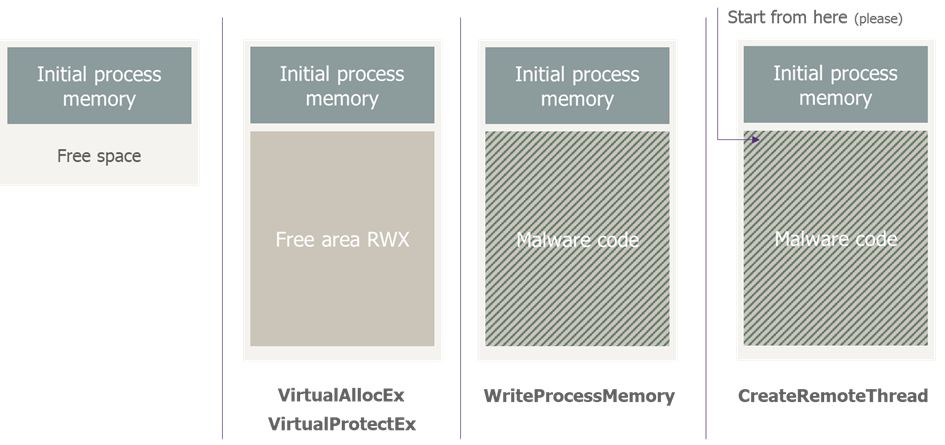
\includegraphics[scale=0.9]{dequeker_standard_process_injection_pattern.png}
\caption{Standard process Injection pattern \autocite{Dequeker:2023}}
\end{figure}
 

\subsubsection{\textcite{S12h4ck:2023a}}
\textbf{\citetitle{S12h4ck:2023a}}:  This paper utilizes NT APIs related to shared memory to stealthily inject shellcode into the address space of a target process and execute it via starting a remote thread. The goal is to bypass monitoring of common code injection techniques.

\textbf{Keywords}: NT APIs, Code injection, Shared memory, Memory section, Remote thread, Shellcode, Stealth.

Here is a summary of the process injection technique discussed in this paper:

Category:
\begin{itemize}
\item Victim Selection: Targeted Injection
\item Code Execution: Concurrent Execution
\end{itemize}

Advantages:
\begin{itemize}
\item Uses lesser-known NT APIs that may bypass hooks on common injection APIs
\item Allocates payload in shared memory section stealthily
\end{itemize}

Bypass Techniques:
\begin{itemize}
\item Avoids common process injection APIs
\item Creates memory section accessible to target process
\item Starts thread in target process pointed to payload
\item Aims to blend in to legitimate remote thread creation
\end{itemize}

Special Techniques:
\begin{itemize}
\item Uses NtCreateSection to allocate payload in shared memory
\item Maps view of section into target process via NtMapViewOfSection
\item Starts remote thread in target directed at payload view
\end{itemize}


\href{https://github.com/elddy/Windows-NTAPI-Injector}{GitHub.com Windows-NTAPI-Injector}

\href{https://gist.github.com/WKL-Sec/96e17188e4c159c2cdf7ff2c111130cc#file-local-c}{GitHub.com Injector examples in C}


\subsubsection{\textcite{S12h4ck:2023b}}
\textbf{\citetitle{S12h4ck:2023b}}:  So, picture this: you’re in a digital realm where security is paramount, and there’s an ongoing battle between the good guys and the cyber-criminals. Process injection is like a ninja move in this digital showdown, and these “random RWX memory spaces” are the secret hideouts where the action unfolds.

\textbf{Keywords}: Process injection, Code injection, Shellcode injection, Memory scanning, RWX pages, Random injection regions

This C++ code appears to be a Windows application that performs process injection using a specific shellcode into processes that have memory regions marked as PAGE\_EXECUTE\_READWRITE. Process injection is a technique used in various scenarios, including security research and, unfortunately, malicious activities.


In summary, this paper discusses a more advanced targeted injection technique that aims to be stealthier by finding unpredictable RWX memory areas to inject shellcode and start execution from. The goal is to bypass defences through unusual allocation and execution methods.

Here is a summary of the process injection technique discussed in this paper:

Category:
\begin{itemize}
\item Victim Selection: Targeted Injection
\item Code Execution: Concurrent Execution
\end{itemize}

Advantages:
\begin{itemize}
\item Finds random RWX memory regions to inject code, making it stealthier and more unpredictable
\item Bypasses some defences that monitor common injection techniques
\end{itemize}

Bypass Techniques:
\begin{itemize}
\item Uses uncommon Windows APIs like VirtualQueryEx to scan process memory
\item Looks for rare RWX regions instead of predictable allocated memory
\item Makes code execution flow appear valid via CreateRemoteThread
\end{itemize}

Special Techniques:
\begin{itemize}
\item Scans process memory regions to find random RWX areas
\item Uses WTSEnumerateProcesses to get list of running processes
\item Writes shellcode to RWX region found then starts new thread there
\end{itemize}


\href{https://www.unknowncheats.me/forum/anti-cheat-bypass/286274-internal-detection-vectors-bypass.html}{internal detection vectors bypass}


\subsubsection{\textcite{smellyvx:2021}}

\textbf{\citetitle{smellyvx:2021}}:

\textbf{Keywords}:  Dynamic syscall resolution, PE headers, Pseudo-disassembly, Position independent code, Shellcode injection, Process injection.

Explains weaknesses of relying on hardcoded syscalls for malware and red team tools. Vulnerable to breakage across OS versions.

Discusses dynamically resolving syscalls from ntdll.dll export table at runtime to build a position independent call table.

Walks PE headers to find the export table. Pseudo-disassembles functions to extract syscall numbers.

Builds a table of syscalls without any dependencies or imports. Uses assembled shellcode to invoke them.

Proof-of-concept demonstrates resolving APIs and using them to perform process injection. Avoids hardcoded dependencies.

Differences from Previous Articles:

Focuses on fully dynamic syscall resolution unlike static definitions used before.

Aims for total position independence rather than relying on imports.

Disassembles export table to find syscalls instead of hardcoded values.

Builds entire call table at runtime to avoid breakages across OS versions.

Uses handwritten assembly stub to invoke syscalls.

This technique is more advanced because it completely decouples dependency on any imports or static syscall definitions. By pseudo-disassembling functions and extracting the values, it can adapt to any Windows version. The position independent call table and assembled shellcode allow executing payloads without relying on hardcoded links. This makes the resulting program highly portable and resilient.



\section{Return of the Jedi: EDRs Response to an Evolving Threat Landscape}

Review EDR capabilities.  To counter process injection attacts EDR systems can:

\begin{itemize}
\item Static Monitoring of specific DLLs or System Calls: The first level of protection against process injection attack techiques is
  scan processes \ldots
\item Behavioural Analysis: User and entity behaviour analytics (UEBA) are being introduced into XDR tools \ldots
\item Anomaly detection: \autocite{Pek:2016} \ldots
\item Machine Learning techniques: \autocite{Wang:2022}
\end{itemize}



\subsection{Endpoint Security: EDR}

\subsubsection{\textcite{Hayes:2023}}
\textbf{\citetitle{Hayes:2023}}:  Endpoint detection and response (EDR) is a cybersecurity solution that captures all endpoint activity and leverages advanced analytics to provide real-time visibility into the health of all endpoints; detect anomalous activity; alert the information security (Infosec) team to events; and provide remediation suggestions and capabilities to respond, stop an attack in progress or limit its spread.

Endpoint detection and response solutions have the following capabilities:

\begin{itemize}
\item	Endpoint monitoring and event recording
\item	Data search, investigation and threat hunting
\item	Alert triage or suspicious activity validation
\item	Suspicious activity detection
\item	Data analysis
\item	Actionable intelligence to support response
\item	Remediation
\end{itemize}

Managed detection and response (MDR) is endpoint security “as a service.” This  service manages endpoint security technologies for organizations which includes EDR. Service capabilities typically include: :

\begin{itemize}
\item	Continuous monitoring
\item	Threat hunting
\item	Prioritization of threats and alerts
\item	Managed investigation services
\item	Guided response
\item	Managed remediation
\end{itemize}

The main benefit of MDR is that it helps rapidly identify and limit the impact of threats without the need for additional staffing. This is especially important given the global shortage of highly skilled cybersecurity professionals and the related skills gap, particularly as it relates to protection of cloud-based systems and assets.

Extended detection and response (XDR) streamlines security data ingestion, analysis and workflows across an organization’s entire security stack, enhancing visibility around hidden and advanced security threats and unifying the response.

An XDR platform collects and correlates data from across the infrastructure so it can improve threat visibility across the enterprise, accelerate security operations and reduce risk. XDR analyzes, prioritizes and streamlines this data, so it can be delivered to security teams in a normalized format through a single, consolidated console.
XDR platforms typically offer the following capabilities:

\begin{itemize}
\item	Diverse, multi-domain security telemetry
\item	Threat-focused event analysis
\item	Threat detection and prioritization of data fidelity
\item	Data search, investigation and threat hunting across multi-domain telemetry
\item	Response to mitigate and remediate the threat
\end{itemize}


\subsubsection{Types of analysis}
he article suggests that the MRm-DLDet framework improves on older techniques of memory-resident malware detection that rely on static and dynamic analysis methods. Static analysis methods involve analyzing the code and structure of a program without executing it, while dynamic analysis methods involve executing the program and observing its behavior. However, these methods may not be effective in detecting memory-resident malware, which executes only in memory and leaves little evidence on disk. 

\subsection{What is on offer and where are EDRs failing}

\subsubsection{\textcite{Lyles:2022}}
\textbf{\citetitle{Lyles:2022}}: As signature-based malware detection techniques mature, malware authors have been forced to leave fewer footprints on target machines. Malicious activity can be conducted by chaining together benign, built-in functions in subversive ways. Because the functions are native to the host system, attackers can slip under the radar of signature filtering tools such as YARA. To address this challenge, we utilize the Volatility memory forensics framework to measure and characterize typical in-memory behavior, then observe the deviations from normal use that may indicate a compromise. We demonstrate that processes have characteristic memory footprints, and that machine learning models can flag malicious behavior as anomalous.

The paper categorizes malware detection techniques into two types: 

1. Traditional detection techniques: These techniques generate signatures that can identify known types of malware based on their file contents. Examples include hashing the entire executable, signature-based n-gram models, and other anomaly detection methods.

2. Machine learning aided malware detection: This approach utilizes machine learning models to detect malicious behavior in memory images. The models are trained on extracted measurements from memory images using the Volatility memory forensics framework.

Compared to traditional detection techniques, machine learning aided malware detection has several advantages. First, it can detect fileless or memory-based attacks that traditional techniques may miss. Second, it can identify deviations from normal in-memory behavior that may indicate a compromise. Third, it can flag suspicious processes even when they are using benign, built-in functions in subversive ways. Finally, it can automate the detection process, making it more efficient and effective.

The paper suggests that deviations from normal in-memory behavior are key indicators for detecting compromises. Specifically, the deviations that are best for detecting compromises include anomalies in memory footprints and behaviors of processes. By characterizing typical in-memory behavior and observing deviations from normal use, machine learning models can flag malicious behavior as anomalous. This approach allows for the identification of suspicious processes, even when they are using benign, built-in functions in subversive ways, thus providing a more comprehensive and effective method for detecting compromises.

Yes, in the context of machine learning aided malware detection, it is essential to train the AI model on normal process behavior before it can effectively detect anomalies. By training the model on normal behavior, it learns to recognize patterns and characteristics that are typical of benign processes. Once the model has been trained on normal behavior, it can then identify deviations from this normal behavior as potential anomalies or indicators of compromise. This approach allows the AI model to distinguish between normal and abnormal behavior, enabling it to effectively detect malicious activity in memory images.

The paper primarily utilizes a supervised learning approach, specifically employing random forest classifier models to analyze and detect malicious behavior in memory images. Supervised learning involves training the model on labeled data, where the input features (in this case, measurements extracted from memory images) are used to predict the output (normal or malicious behavior).

\subsection{We're not going to avoid every injection attack}

\subsubsection{\textcite{Zengy:2022}}
\textbf{\citetitle{Zengy:2022}}:  System auditing provides a low-level view into cyber threats by monitoring system entity interactions. In response to advanced cyber-attacks, one prevalent solution is to apply data provenance analysis on audit records to search for anomalies (anomalous behaviors) or specifications of known attacks. However, existing approaches suffer from several limitations: 1) generating high volumes of false alarms, 2) relying on expert knowledge, or 3) producing coarse-grained detection signals. In this paper, we recognize the structural similarity between threat detection in cybersecurity and recommendation in information retrieval. By mapping security concepts of system entity interactions to recommendation concepts of user-item interactions, we identify cyber threats by predicting the preferences of a system entity on its interactive entities. Furthermore, inspired by the recent advances in modeling high-order connectivity via item side information in the recommendation, we transfer the insight to cyber threat analysis and customize an automated detection system, SHADEWATCHER. It fulfills the potential of high-order information in audit records via graph neural networks to improve detection effectiveness. Besides, we equip SHADEWATCHER with dynamic updates towards better generalization to false alarms. In our evaluation against both real-life and simulated cyber-attack scenarios, SHADEWATCHER shows its advantage in identifying threats with high precision and recall rates. Moreover, SHADEWATCHER is capable of pinpointing threats from nearly a million system entity interactions within seconds.


\subsection{What could detection systems look for}

\subsubsection{\textcite{Pek:2016} Looking at memory paging of compromised processes}
\textbf{\citetitle{Pek:2016}}: Design and implement Membrane, a memory forensics tool to detect code loading behavior by stealthy malware. Instead of trying to detect the code loading itself, we focus on the changes it causes on the memory paging of the Windows operating system. As our method focuses on the anomalies caused by code loading, we are able to detect a wide range of code loading techniques. Our results indicate that we can detect code loading malware behavior with 86.98\% success in most cases, including advanced targeted attacks. Our method is generic enough and hence could significantly raise the bar for attackers to remain stealthy and persist for an extended period of time.


\subsubsection{\textcite{Liu:2023}}
\textbf{\citetitle{Liu:2023}}:  Cyber attackers have constantly updated their attack techniques to evade antivirus software detection in recent years. One popular evasion method is to execute malicious code and perform malicious actions only in memory. Malicious programs that use this attack method are called memory-resident malware, with excellent evasion capability, and have posed huge threats to cyber security. Traditional static and dynamic methods are not effective in detecting memory-resident malware. In addition, existing memory forensics detection solutions perform unsatisfactorily in detection rate and depend on massive expert knowledge in memory analysis. This paper proposes MRm-DLDet, a state-of-the-art memory-resident malware detection framework, to overcome these drawbacks. MRm-DLDet first builds a virtual machine environment and captures memory dumps, then creatively processes the memory dumps into RGB images using a pre-processing technique that combines deduplication and ultra-high resolution image cropping, followed by our neural network MRmNet in MRm-DLDet to fully extract high-dimensional features from memory dump files and detect them. MRmNet receives the labeled sub-images of the cropped high-resolution RGB images as input of ResNet-18, which extracts the features of the sub-images. Then trains a network of gated recurrent units with an attention mechanism. Finally, it determines whether a program is memory-resident malware based on the detection results of each sub-image through a specially designed voting layer. We created a high-quality dataset consisting of 2,060 benign and memory-resident programs. In other words, the dataset contains 1,287,500 labeled sub-images cut from the MRm-DLDet transformed ultra-high resolution RGB images. We implement MRm-DLDet for Windows 10, and it performs better than the latest methods, with a detection accuracy of up to 98.34\% . Moreover, we measured the effects of mimicry and adversarial attacks on MRm-DLDet, and the experimental results demonstrated the robustness of MRm-DLDet.

The article presents a memory-resident malware detection framework called MRm-DLDet, which utilizes memory forensics and deep neural network to detect malicious code and actions that occur only in memory, evading traditional antivirus software detection. The framework is evaluated using various datasets and compared with other state-of-the-art methods, showing promising results in terms of accuracy, precision, recall, and F1-score. The authors suggest that the framework can be used to improve cybersecurity measures against evolving cyber attack techniques.

Yes, the memory dump can be produced while the process is active. In fact, the article describes how the authors generated memory dumps by automating the process using the vmrun utility to control a Windows 10 virtual machine. The virtual machine was rolled back to its initial state before running each sample, and the memory dump was captured using the vmrun utility's 'createSnap' operation, which dumps the VM's memory state to a file. The authors suggest that most malicious behavior can be observed within the first two minutes of execution, so each malicious sample was given two minutes to initialize and execute before the memory dump was captured.

The process described in the article for generating memory dumps and using them for memory-resident malware detection may not be practical for running on all computers in a corporate network. The process involves automating the memory dump generation process using a virtual machine, which may not be feasible for all computers in a corporate network. Additionally, the process may require significant computational resources and time to generate and analyze memory dumps, which may not be practical for large-scale deployment. 

However, the authors suggest that the framework can be deployed on client devices to detect suspicious PE files according to user requirements, and return the detection results in real-time. This approach may be more practical for corporate networks, as it allows for targeted detection of suspicious files and reduces the computational resources required for memory dump analysis.

\subsection{It's a bit late, but some feedback to the vendor is in order}

\subsubsection{\textcite{Zeng:2021}}
\textbf{\citetitle{Zeng:2021}}:  Endpoint monitoring solutions are widely deployed in today's enterprise environments to support advanced attack detection and investigation. These monitors continuously record system-level activities as audit logs and provide deep visibility into security incidents. Unfortunately, to recognize behaviors of interest and detect potential threats, cyber analysts face a semantic gap between low-level audit events and high-level system behaviors. To bridge this gap, existing work largely matches streams of audit logs against a knowledge base of rules that describe behaviors. However, specifying such rules heavily relies on expert knowledge. In this paper, we present WATSON, an automated approach to abstracting behaviors by inferring and aggregating the semantics of audit events. WATSON uncovers the semantics of events through their usage context in audit logs. By extracting behaviors as connected system operations, WATSON then combines event semantics as the representation of behaviors. To reduce analysis workload, WATSON further clusters semantically similar behaviors and distinguishes the representatives for analyst investigation. In our evaluation against both benign and malicious behaviors, WATSON exhibits high accuracy for behavior abstraction. Moreover, WATSON can reduce analysis workload by two orders of magnitude for attack investigation.


\subsection{But will it be good enough}

\subsubsection{\textcite{Wang:2022}}
\textbf{\citetitle{Wang:2022}}: New malware increasingly adopts novel fileless techniques to evade detection from antivirus programs. Process injection is one of the most popular fileless attack techniques. This technique makes malware more stealthy by writing malicious code into memory space and reusing the name and port of the host process. It is difficult for traditional security software to detect and intercept process injections due to the stealthiness of its behavior. We propose a novel framework called ProcGuard for detecting process injection behaviors. This framework collects sensitive function call information of typical process injection. Then we perform a fine-grained analysis of process injection behavior based on the function call chain characteristics of the program, and we also use the improved RCNN network to enhance API analysis on the tampered memory segments. We combine API analysis with deep learning to determine whether a process injection attack has been executed. We collect a large number of malicious samples with process injection behavior and construct a dataset for evaluating the effectiveness of ProcGuard. The experimental results demonstrate that it achieves an accuracy of 81.58\% with a lower false-positive rate compared to other systems. In addition, we also evaluate the detection time and runtime performance loss metrics of ProcGuard, both of which are improved compared to previous detection tools.

% Section 3 an investigation into the Mockingjay attack and against a recently published paper ``Procguard'' \cite:{Wang:2022} and asks weather this attack method would lickly be caught.
\section{Case Study: Introducing MockingJay; New Process Injection Attacks}


\href{https://www.securityjoes.com/post/process-mockingjay-echoing-rwx-in-userland-to-achieve-code-execution}{Mockingjay echoing in userland to achieve code execution}

\href{https://www.linkedin.com/posts/john-stigerwalt-90a9b4110_mockingjay-memory-allocation-primitive-activity-7083050050158743552-Hgyw}{mockingjay memory allocation primative}

\href{https://whiteknightlabs.com/2023/07/06/mockingjay-memory-allocation-primitive/}{white knights mocking jay}

The Mockingjay  attack targets trusted and legitimate processes runing on a sytem.  


%\subsection{Real-world examples of malware employing process injection on Windows}
\subsection{Context: Detailed analysis of new process injection attacks.}

\citetitle{smellyvx:2021} \autocite{smellyvx:2021}
\subsubsection{\textcite{Peixoto:2023}}
\textbf{\citetitle{Peixoto:2023}}: Throughout the blog post, we will delve into various process injection techniques employed by attackers to bypass security controls and gain unauthorized access. We will address the challenges presented by EDRs and XDRs, emphasizing the importance of understanding and mitigating the risks associated with process injection. Additionally, we will share insights gained from our research, including the development of our own process injection technique. We will highlight the capabilities and implications of this technique, shedding light on its effectiveness, potential impact and detection opportunities for defenders.

\textbf{Why is this technique important?}: It's a new potential security vulnerability. It is a process injection
technique utilised byattackers to deceive robust security products in a corporate environment, such as ``EDRS'' and \textbf{XDRS}.

Process is designed to bypass security controls to gain unauthorised access.


Summary:

Identifies that EDRs hook common injection APIs like VirtualAllocEx. Aims to find alternate injection methods.
Discovers a vulnerable DLL with a default RWX code section that can be leveraged.
Uses the RWX section to inject shellcode into same and remote processes without typical allocation or permission APIs.
Tests self-injection into a process and remote injection into ssh.exe process as proof-of-concepts.

\textbf{Keywords}: Process injection, EDR evasion, RWX permissions , Shellcode injection. Remote process injection

Differences from Previous Articles:

Novel technique using default vulnerable DLL instead of typical injection workflows
Eliminates usage of memory allocation and permission APIs typically monitored by EDRs
Leverages RWX section to avoid setting execute permissions after allocation
No need to explicitly create any threads for execution unlike other methods
Tests both self-injection and sophisticated remote injection with ssh.exe
This is an advanced technique because it demonstrates a stealthy way to perform process injection using a permission misconfiguration instead of easily detectable Windows APIs. By locating an existing RWX code section, it bypasses allocation and permission hooks in EDRs. The remote ssh.exe injection also runs shellcode seamlessly without starting threads. The abuse of privileged sections gives it an element of novelty over typical injection tactics.


\subsection{Alternatives: how these attacks could potentially evade EDR}

\subsubsection{It couldn't happen to me/The CISO and current state of malware attacks on Windows.}

\subsubsection{\textcite{CISA:2023a}}
\textbf{\citetitle{CISA:2023a}}:  CVE-2023-4966 is a software vulnerability found in Citrix NetScaler ADC and NetScaler Gateway appliances with exploitation activity identified as early as August 2023. This vulnerability provides threat actors, including LockBit 3.0 ransomware affiliates, the capability to bypass MFA [T1556.006] and hijack legitimate user sessions [T1563].

After acquiring access to valid cookies, LockBit 3.0 affiliates establish an authenticated session within the NetScaler appliance without a username, password, or access to MFA tokens [T1539]. Affiliates acquire this by sending an HTTP GET request with a crafted HTTP Host header, leading to a vulnerable appliance returning system memory information [T1082]. The information obtained through this exploit contains a valid NetScaler AAA session cookie.

Threat Actor Activity
Malware identified in this campaign is generated beginning with the execution of a PowerShell script (123.ps1) which concatenates two base64 strings together, converts them to bytes, and writes them to the designated file path.

\begin{verbatim}
$y = "TVqQAAMA...<long base64 string>"
$x = "RyEHABFQ...<long base64 string>"
$filePath = "C:\Users\Public\adobelib.dll"
$fileBytes = [System.Convert]::FromBase64String($y + $x)
[System.IO.File]::WriteAllBytes($filePath, $fileBytes)
\end{verbatim}

The resulting file (adobelib.dll) is then executed by the PowerShell script using rundll32.

\begin{verbatim}
rundll32 C:\Users\Public\adobelib.dll,main <104 hex char key>
\end{verbatim}

The Dynamic Link Library (DLL) will not execute correctly without the 104 hex character key. Following execution, the DLL attempts to send a POST request to https://adobe-us-updatefiles[.]digital/index.php which resolves to IP addresses 172.67.129[.]176 and 104.21.1[.]180 as of November 16, 2023. Although adobelib.dll and the adobe-us-updatefiles[.]digital have the appearance of legitimacy, the file and domain have no association with legitimate Adobe software and no identified interaction with the software.

Other observed activities include the use of a variety of TTPs commonly associated with ransomware activity. For example, LockBit 3.0 affiliates have been observed using AnyDesk and Splashtop remote management and monitoring (RMM), Batch and PowerShell scripts, the execution of HTA files using the Windows native utility mshta.exe and other common software tools typically associated with ransomware incidents.

\subsubsection{\textcite{CVE-2023-3467}}
\textbf{\citetitle{CVE-2023-3467}}: 


\subsubsection{\textcite{CVE-2023-3519}}
\textbf{\citetitle{CVE-2023-3519}}: 


%\subsection{Analysis of the impact and consequences of these incidents}
\subsection{Significance of the use case in assessing and improving the organization's cybersecurity measures.}


\subsubsection{\textcite{CISA:2023}: Understanding the enemy}
\textbf{\citetitle{CISA:2023}}


\subsubsection{\textcite{Wang:2020}}
\textbf{\citetitle{Wang:2020}}:  To subvert recent advances in perimeter and host security, the attacker community has developed and employed various attack vectors to make a malware much stealthier than before to penetrate the target system and prolong its presence. Advanced malware or "stealthy malware" makes use of various techniques to impersonate or abuse benign applications and legitimate system tools to minimize its footprints in the target system. Thus, it is difficult for traditional detection tools, such as malware scanners, to detect it, as the malware normally does not expose its malicious payload in a file and hides its malicious behaviors among the benign behaviors of the processes. In this paper, we present PROVDETECTOR, a provenance-based approach for detecting stealthy malware. Our insight behind the PROVDETECTOR approach is that although stealthy malware attempts to blend into benign processes, the malicious behaviors inevitably interact with the underlying operating system (OS), which will be exposed to and captured by provenance monitoring. Based on this intuition, PROVDETECTOR first employs a novel selection algorithm to identify possible malicious parts in the OS-level provenance data of a process. It then applies a neural embedding and machine learning pipeline to automatically detect any behavior that deviates significantly from normal behaviors. We evaluate our approach on a large provenance dataset from an enterprise network and demonstrate that it achieves very high detection performance of stealthy malware (an average F1 score of 0.974). Further, we conduct thorough interpretability studies to understand the internals of the learned machine learning models.

\textbf{Keywords}: Data provenance, Process injection, Anomaly detection, Interpretability, Causality reasoning.

Category: Targeted Injection, Concurrent Execution

Summary and analysis of the approach for detecting stealthy malware using provenance data.  The article uses targeted selection of anomalous provenance subgraphs and transparent ML models over them to provide interpretable reasoning for stealthy malware detection.

The article proposes PROVDETECTOR, an anomaly detection system that models normal program behavior using kernel-level provenance graphs to detect stealthy malware that tries to blend in.

It selects the top 20 most uncommon causal paths from each process's provenance graph to focus on anomalous parts of execution. These paths are embedded using document embeddings and fed into a Local Outlier Factor model to identify outliers.

\begin{enumerate}
\item Advantages:

  \begin{enumerate}
  \item Uses full causality chains rather than single events
  \item Focuses modeling on uncommon behavior more likely to be malicious
  \item Achieves very high accuracy (0.974 F1 score)
  \end{enumerate}

\item Bypass Techniques:

  \begin{enumerate}
  \item Relies on uncommon paths invisible to simpler models
  \item Contextual embedding detects semantic mimicry
  \end{enumerate}

\item Special Techniques:

  \begin{enumerate}
  \item Path rarity for feature selection
  \item Document embeddings for causality chains
  \item Local outlier detection without distribution assumptions
  \end{enumerate}
\end{enumerate}

The approach explicitly tries to provide interpretability on why a process is flagged malicious. The embedding model learns holistic paths instead of individual nodes. Local feature importance measures like LIME are used to indicate key causal dependencies that lead to a detection. This transparency helps analysts trust the system.


\subsubsection{\textcite{Inam:2023}: Provenance-based system auditing and how it could improve EDR malware detection}
\textbf{\citetitle{Inam:2023}}:  Auditing, a central pillar of operating system security, has only recently come into its own as an active area of public research. This resurgent interest is due in large part to the notion of data provenance, a technique that iteratively parses audit log entries into a dependency graph that explains the history of system execution. Provenance facilitates precise threat detection and investigation through causal analysis of sophisticated intrusion behaviors. However, the absence of a foundational audit literature, combined with the rapid publication of recent findings, makes it difficult to gain a holistic picture of advancements and open challenges in the area.In this work, we survey and categorize the provenance-based system auditing literature, distilling contributions into a layered taxonomy based on the audit log capture and analysis pipeline. Recognizing that the Reduction Layer remains a key obstacle to the further proliferation of causal analysis technologies, we delve further on this issue by conducting an ambitious independent evaluation of 8 exemplar reduction techniques against the recently-released DARPA Transparent Computing datasets. Our experiments uncover that past approaches frequently prune an overlapping set of activities from audit logs, reducing the synergistic benefits from applying them in tandem; further, we observe an inverse relation between storage efficiency and anomaly detection performance. However, we also observe that log reduction techniques are able to synergize effectively with data compression, potentially reducing log retention costs by multiple orders of magnitude. We conclude by discussing promising future directions for the field.

Auditing captures documentary evidence of the events that took place on a target system. Today, most operating systems come with auditing frameworks, such as the Linux Audit Subsytem [91], Event Tracing for Windows (ETW) [109], and FreeBSD’s DTrace [110]. These frameworks use audit hooks and system call interception to monitor accesses between system subjects (e.g., processes) and system objects (e.g., files, sockets, pipes, etc.). Configured properly, audit logs can contain enough information to establish what events occurred on the system and how and who caused those events [111]. Au- diting thus complements purely post-mortem forensic methods such as disk [112], memory [113], and malware analysis [114].


Provenance-based system auditing refers to the capture and analysis of detailed logs that track the history and dependencies between system events and entities. This allows reconstructing the chain of events leading up to an attack (backtracing) or the ramifications of an attack (forward tracing).

Provenance auditing builds contextual graphs of system execution that can detect complex malware behaviors often missed by traditional EDR monitoring. This improves detection rates and investigation efficiency.

Compared to \autocite{Wang:2020} this approach uses a more complex LSTM-based detection model that is harder to interpret. \textcite{Wang:2020}'s use of simple embedding and outlier detection makes the provenance-based causality reasoning more scrutable.


The article categorizes provenance-based auditing techniques into 5 layers:

\begin{itemize}
\item Capture - logs system events at various levels like kernel, application, middleware
\item Reduction - removes irrelevant events to improve storage and analysis
\item Infrastructure - stores and queries audit data
\item Detection - analyzes logs to identify indicators of attack
\item Investigation - interfaces for analysts to inspect and interpret audit data
\item The detection layer is where EDR systems operate. The article notes two weaknesses of current EDR heuristic and anomaly detection approaches:
\end{itemize}

\begin{itemize}
\item They focus on events in a single process rather than cross-process causal dependencies. Provenance graphs better represent multistage attacks spanning processes.
\item They suffer from high false positive rates leading to alert fatigue. Provenance provides intrinsic context to help dismiss benign alerts.
\end{itemize}

By leveraging causality analysis and historical context, provenance-based auditing could improve EDR detection of sophisticated malware attacks in the following ways:

\begin{enumerate}
\item Represent multistage attack behaviors across processes
\item Reduce false positives by explaining attack context
\item Detect attack pattern variants based on causal dependencies
\item Identify root causes and ramifications of an attack
\end{enumerate}



\begin{figure}[ht]
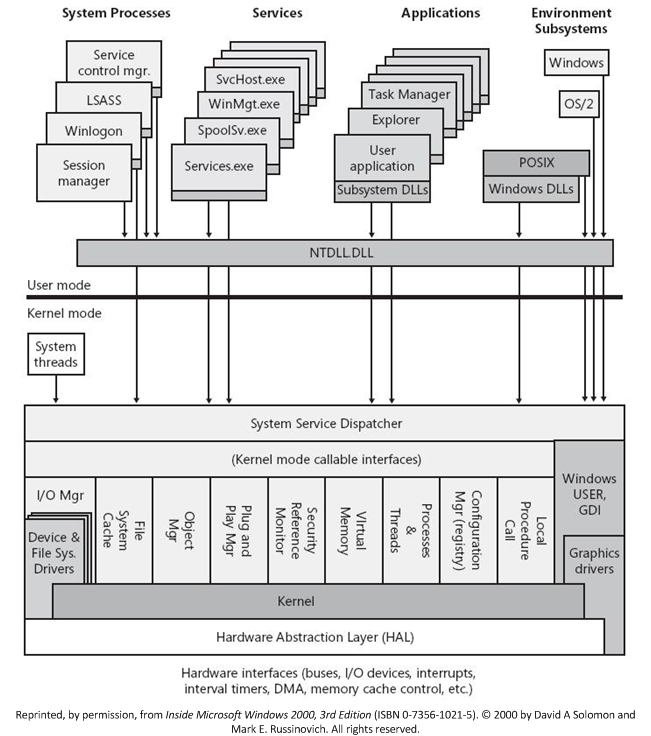
\includegraphics[scale=0.4]{ms_hardware_interfaces.png}
\caption{MS Hardware Interfaces}
\end{figure}

\printbibliography

\end{document}

%%% Local Variables:
%%% mode: latex
%%% TeX-master: t
%%% End: